%%
%% Automatically generated file from DocOnce source
%% (https://github.com/hplgit/doconce/)
%%
%%


%-------------------- begin preamble ----------------------

\documentclass[%
twoside,                 % oneside: electronic viewing, twoside: printing
final,                   % or draft (marks overfull hboxes, figures with paths)
10pt]{article}

\listfiles               % print all files needed to compile this document

\usepackage{relsize,makeidx,color,setspace,amsmath,amsfonts}
\usepackage[table]{xcolor}
\usepackage{bm,microtype}

\usepackage{graphicx}

\usepackage[T1]{fontenc}
%\usepackage[latin1]{inputenc}
\usepackage{ucs}
\usepackage[utf8x]{inputenc}

\usepackage{lmodern}         % Latin Modern fonts derived from Computer Modern

% Hyperlinks in PDF:
\definecolor{linkcolor}{rgb}{0,0,0.4}
\usepackage{hyperref}
\hypersetup{
    breaklinks=true,
    colorlinks=true,
    linkcolor=linkcolor,
    urlcolor=linkcolor,
    citecolor=black,
    filecolor=black,
    %filecolor=blue,
    pdfmenubar=true,
    pdftoolbar=true,
    bookmarksdepth=3   % Uncomment (and tweak) for PDF bookmarks with more levels than the TOC
    }
%\hyperbaseurl{}   % hyperlinks are relative to this root

\setcounter{tocdepth}{2}  % number chapter, section, subsection

% Tricks for having figures close to where they are defined:
% 1. define less restrictive rules for where to put figures
\setcounter{topnumber}{2}
\setcounter{bottomnumber}{2}
\setcounter{totalnumber}{4}
\renewcommand{\topfraction}{0.85}
\renewcommand{\bottomfraction}{0.85}
\renewcommand{\textfraction}{0.15}
\renewcommand{\floatpagefraction}{0.7}
% 2. ensure all figures are flushed before next section
\usepackage[section]{placeins}
% 3. enable begin{figure}[H] (often leads to ugly pagebreaks)
%\usepackage{float}\restylefloat{figure}

\usepackage[framemethod=TikZ]{mdframed}

% --- begin definitions of admonition environments ---

% --- end of definitions of admonition environments ---

% prevent orhpans and widows
\clubpenalty = 10000
\widowpenalty = 10000

% --- end of standard preamble for documents ---


% insert custom LaTeX commands...

\raggedbottom
\makeindex

%-------------------- end preamble ----------------------

\begin{document}



% ------------------- main content ----------------------

% Slides for PHY981


% ----------------- title -------------------------

\thispagestyle{empty}

\begin{center}
{\LARGE\bf
\begin{spacing}{1.25}
Nuclear Physics courses, MSU/FRIB theory center and \href{{http://www.nucleartalent.org}}{nuclear TALENT}
\end{spacing}
}
\end{center}

% ----------------- author(s) -------------------------

\begin{center}
{\bf Morten Hjorth-Jensen, National Superconducting Cyclotron Laboratory and Department of Physics and Astronomy, Michigan State University, East Lansing, MI 48824, USA {\&} Department of Physics, University of Oslo, Oslo, Norway${}^{}$} \\ [0mm]
\end{center}

    \begin{center}
% List of all institutions:
\end{center}
    
% ----------------- end author(s) -------------------------

\begin{center} % date
March 31, 2015
\end{center}

\vspace{1cm}


% !split
\subsection*{Motivation}

% --- begin paragraph admon ---
\paragraph{}
\begin{itemize}
\item Develop structured modules which will provide our students with a modern education in nuclear physics

\item Modules/courses should contain a high-level of synchronization

\item A computational perspective is essential

\item They should form a basic curriculum to be integrated with the coming FRIB theory center

\item Coordination with Talent initiative and other Northern American institutions to be elaborated
\end{itemize}

\noindent
We have at MSU a  \href{{https://people.nscl.msu.edu/~witek/Classes/PHY802/NuclPhys802-2015.html}}{basic survey course PHY802}  and three basic nuclear physics courses \href{{http://nuclearstructure.github.io/PHY981/doc/web/course.html}}{structure}, \href{{https://people.nscl.msu.edu/~nunes/phy982/phy982web2015.htm}}{reactions and dynamics}  and \textbf{Nuclear Astrophysics}. These three basic courses
have a duration each  of 30-40 hours (2-3 credits).   

They can be taught as a regular one-semester course or half-semester course. There are also experimental courses not discussed here.
% --- end paragraph admon ---




% !split
\subsection*{The basic courses/modules (theory) taught at MSU}

% --- begin paragraph admon ---
\paragraph{}


% inline figure
\centerline{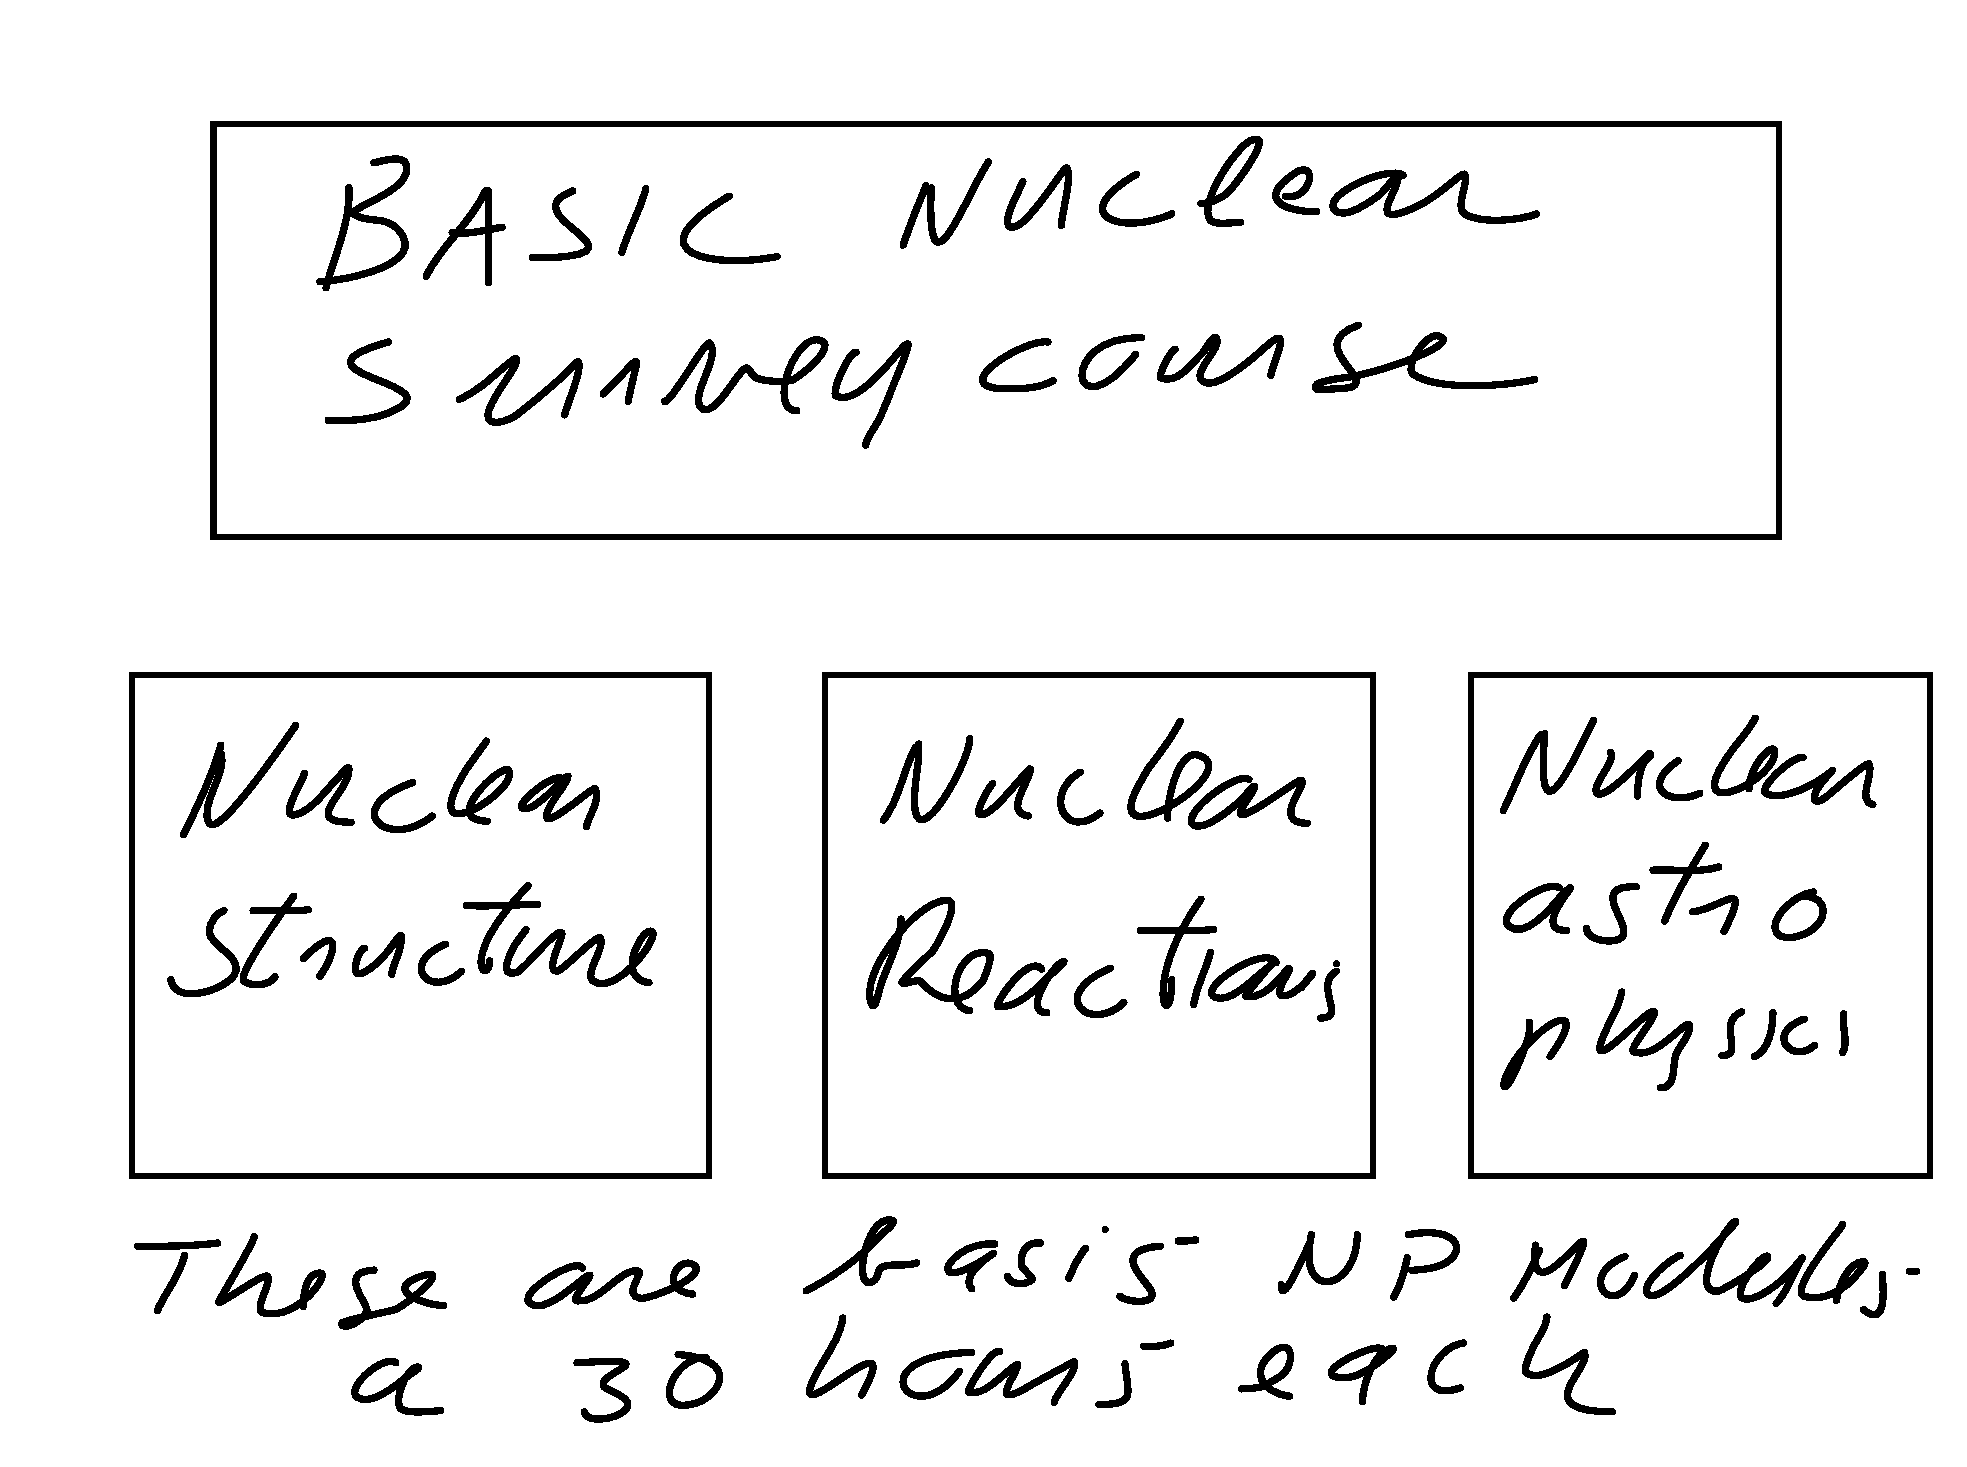
\includegraphics[width=0.5\linewidth]{struct1.pdf}}
% --- end paragraph admon ---




% !split
\subsection*{Nuclear structure course/module  PHY981}

% --- begin paragraph admon ---
\paragraph{}
\begin{itemize}
\item Experimental information

\item Single-particle properties and mean-field

\item second quantization

\item Hartree-Fock theory

\item Nuclear forces (?) Can be taken out since we have an advanced Talent module on this

\item Shell model

\item Transitions (EM and $\beta$-decays

\item Computational elements: build a Hartree-Fock code and/or a shell model code (diagonalization)
\end{itemize}

\noindent
% --- end paragraph admon ---



% !split
\subsection*{Nuclear dynamics course/module  PHY982}

% --- begin paragraph admon ---
\paragraph{}

\begin{itemize}
\item Direct reaction theory and applications

\item Reactions of light and heavy ions, from low to relativistic energies

\item Single-channel scattering

\item Integral forms for scattering. Generalizing to many channels

\item Collective couplings. Single-particle couplings. Coupling to the continuum

\item Transfer reactions. Breakup reactions

\item Adiabatic reaction models. Semiclassical approximations (Eikonal and time-dependent approaches)

\item Capture and fusion reactions

\item R-matrix methods

\item Microscopic models for reactions

\item Several computational exercises
\end{itemize}

\noindent
% --- end paragraph admon ---



% !split
\subsection*{Nuclear astrophysics course/module PHY983}

% --- begin paragraph admon ---
\paragraph{}
\begin{itemize}
\item Neutrinos

\item Equation of state for dense matter

\item Masses - Stability and Decay

\item Reaction Rates

\item Beta decay Rates	

\item The Life of Stars: Stellar burning stages, Hydogen burning, Other burning stages

\item The Death of Stars: Supernovae, Neutron Stars and White Dwarfs

\item Beyond Iron I: r-process, s- and p-process

\item Hydrogen burning at the extremes, the rp process
\end{itemize}

\noindent
% --- end paragraph admon ---




% !split
\subsection*{Advanced  modules, Nuclear Talent}

% --- begin paragraph admon ---
\paragraph{}
\begin{itemize}
\item Nuclear forces (INT 2013, new version 2017)

\item Many-body methods (\textbf{GANIL July 2015})
\begin{itemize}

  \item Many-body perturbation theory

  \item Similarity renormalization group theory

  \item Coupled cluster theory

  \item Green's function theory

  \item FCI (Shell model)
\end{itemize}

\noindent
\end{itemize}

\noindent
% --- end paragraph admon ---





% !split
\subsection*{Advanced  modules, Nuclear Talent}

% --- begin paragraph admon ---
\paragraph{}
\begin{itemize}
\item Few-body methods for nuclear physics (\textbf{ECT* July-August 2015})
\begin{itemize}

 \item Forces and nuclear models

 \item The Faddeev and Faddeev-Yakubowsky Equations

 \item Methods based on Basis expansions

 \item Few-nucleon reactions with external probes
\end{itemize}

\noindent
\end{itemize}

\noindent
% --- end paragraph admon ---




% !split
\subsection*{Advanced  modules, Nuclear Talent}

% --- begin paragraph admon ---
\paragraph{}
\begin{itemize}
\item Density functional theory and self-consistent methods (ECT* 2014 and \textbf{York 2016})

\item Theory for exploring nuclear structure experiments (GANIL 2014)

\item Theory for exploring nuclear reaction experiments (GANIL 2013)
\end{itemize}

\noindent
% --- end paragraph admon ---



% !split
\subsection*{Advanced  modules, Nuclear Talent}

% --- begin paragraph admon ---
\paragraph{}
\begin{itemize}
\item Nuclear theory for astrophysics (MSU 2014 and \textbf{INT 2015})
\begin{itemize}

  \item Stellar evolution, supernova and neutron stars.

  \item Observations and basic properties of neutron stars and supernovae.

  \item Brief review of nuclear forces and nuclear models.

  \item Review of thermodynamics and statistical mechanics.

  \item Basic notions in dense matter theory.

  \item Simple models, the equation of state, and linear response theory.

  \item Homogeneous dense nuclear matter.
\end{itemize}

\noindent
\end{itemize}

\noindent
% --- end paragraph admon ---




% !split
\subsection*{Advanced  modules, Nuclear Talent}

% --- begin paragraph admon ---
\paragraph{}
\begin{itemize}
\item Nuclear theory for astrophysics (MSU 2014 and \textbf{INT 2015})
\begin{itemize}

  \item Homogeneous dense nuclear matter.

  \item Tolman Oppenheimer Volkoff equations and neutron star structure.

  \item Physics at sub-nuclear density and the properties of the neutron star crust.

  \item Superfluidity and superconductivity in neutron stars.

  \item Phase transitions at high density.

  \item Neutrino processes in dense matter and neutron star cooling.

  \item Transport properties of degenerate matter.

  \item Accreting neutron stars.

  \item Supernova neutrinos.

  \item Gravitational waves from neutron star.
\end{itemize}

\noindent
\end{itemize}

\noindent
% --- end paragraph admon ---





% !split
\subsection*{Advanced  modules, Nuclear Talent}

% --- begin paragraph admon ---
\paragraph{}
\begin{itemize}
\item Theoretical approaches to describe  exotic nuclei (planned for 2016, Chalmers, Gothenburg)

\item High-performance computing and computational tools for nuclear physics
\begin{itemize}

  \item ECT* 2012, Shell model and variational Monte Carlo

  \item LANL/ORNL in 2016, Monte Carlo methods 
\end{itemize}

\noindent
\end{itemize}

\noindent
% --- end paragraph admon ---




% !split
\subsection*{Discussion}

% --- begin paragraph admon ---
\paragraph{}
\begin{itemize}
\item How many basic courses can an institution offer, and which courses should be offered?

\item How can the coming FRIB theory center be used to coordinate an advanced training in nuclear physics?

\item Can we integrate the (\emph{ad hoc}) Nuclear Talent courses/initiative  in our education? 

\item Most courses offered are theoretical ones. We need a better coordination between theory and experiment. Should we think of an experimental Talent initiative? 
\end{itemize}

\noindent
% --- end paragraph admon ---








% ------------------- end of main content ---------------


\printindex

\end{document}

